%Be written in English, and submitted as a PDF document with a maximum file size of 5 MB and a guideline length of between 1500 and 3000 words (a few less or more is permissible provided all other requirements are met). You can save Microsoft Word 2016 documents in PDF format, and there are numerous online tools to convert documents to PDF.
%Start with an executive summary or overview section that concisely summarizes the analysis you performed during this project, and the conclusions you reached.
%Continue by describing the data, the process used to explore and analyze it, and the key findings, conclusions, and recommendations you reached.
%Support your conclusions by presenting statistics and visualizations.
%Be submitted by 23:59 on November 25th (UTC) to allow time for peer grading. Note that the deadline shown in the course outline reflects the final deadline for grading your fellow students' reports, not for submitting your own report. 
\documentclass[a4paper,10pt,notitlepage]{article}
\usepackage{helvet}
\usepackage{amsmath}
\usepackage{graphicx}
\usepackage{float}
\usepackage{enumitem}

\renewcommand{\familydefault}{\sfdefault}
\usepackage[scale=.8]{geometry} % use 80% of the page
\usepackage[compact]{titlesec}

\begin{document}

\title{Analysis of home mortgage rate}
\author{Yang Jiao}
\date{\today}

\maketitle

\section{Executive summary}  % or overview
This report presents an analysis of data concerning
how demographics, location, property type, lender and other factors are related to the mortgage rate offered to applicants.
The analysis is based on 200,000 observations of home mortgage disclosure act (HMDA) data, each containing specific characteristics of an loan application.

Potential relationships between characteristics and rate spread were identified. 
A model to predict this rate for loan applications was created.

The author reached the following conclusions:
\begin{itemize}
\item[geo] The location
\end{itemize}

\section{Data exploration and analysis}


\subsection{Individual Feature Statistics}

The targeted value is rate spread, which is discrete numerical value. 
The rate spread distribute from 1.0 to 8.0 and has outliers from 9.0 to 32.0 and then a few cases in 99.0. 
\begin{figure}[H]
\centering
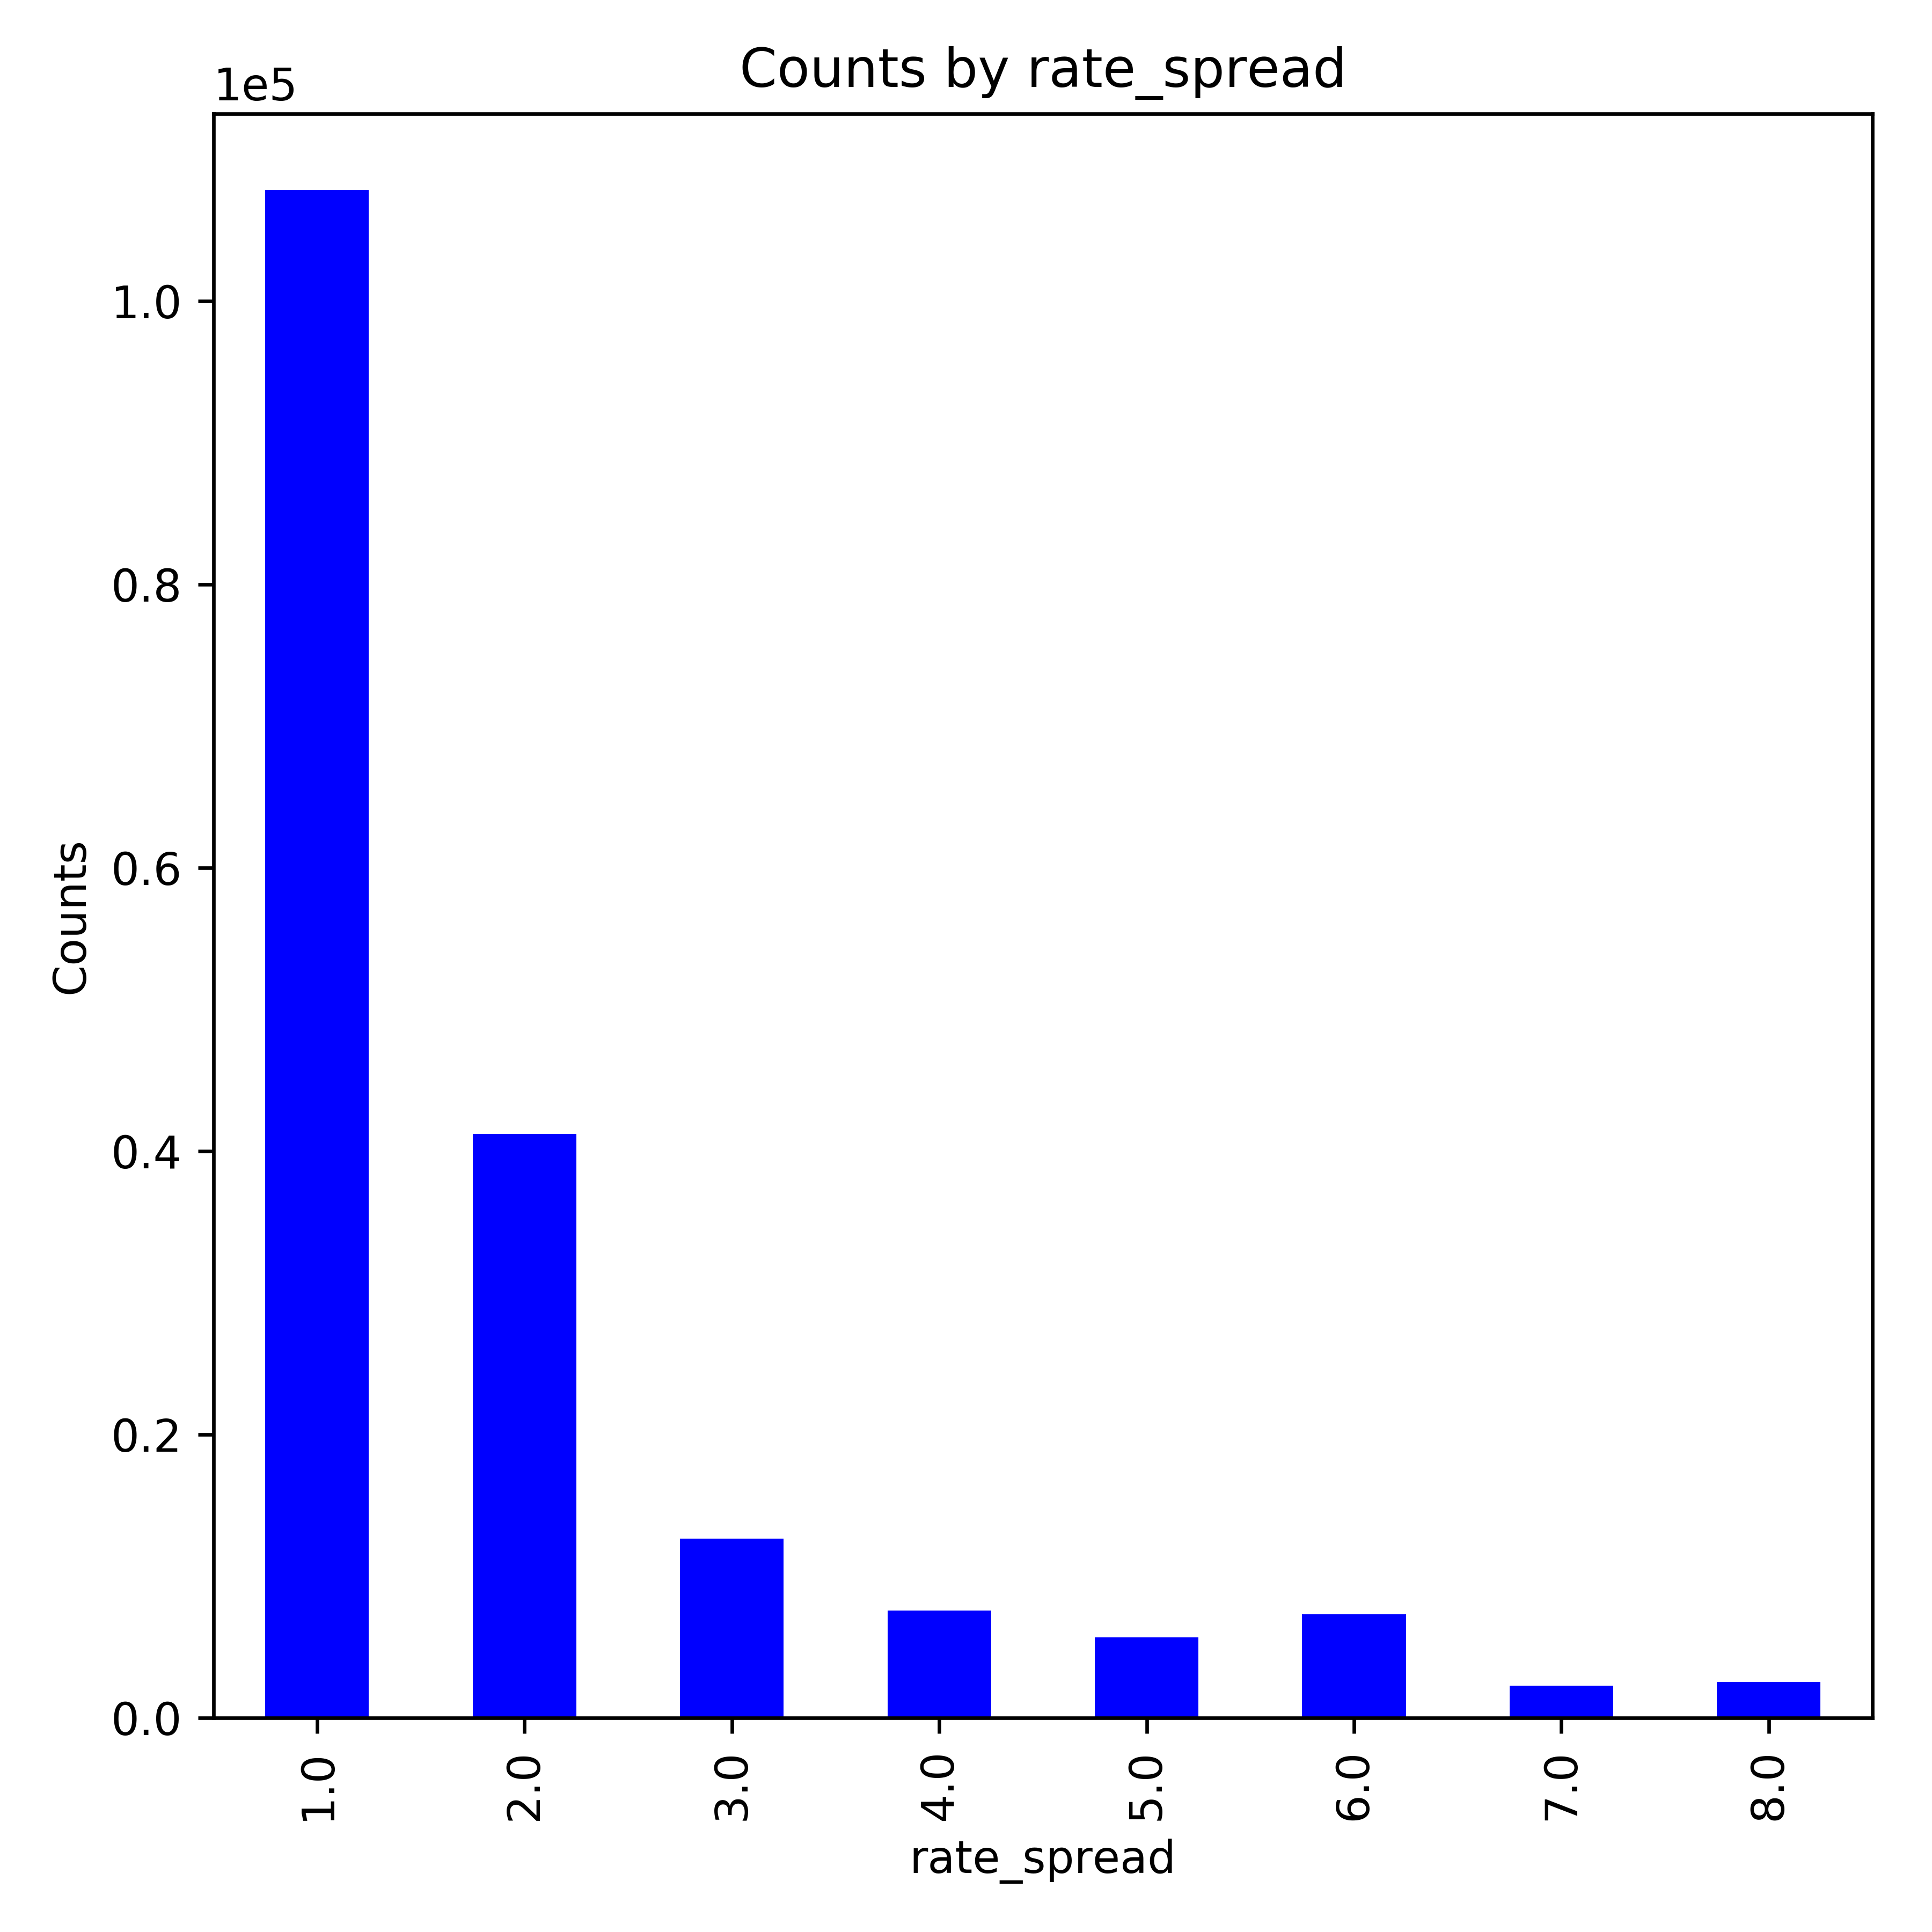
\includegraphics[width=0.6\textwidth]{rate_spread_counts.png}
\caption{The distribution of rate spread in training dataset.}
\label{fig:rate_spread}
\end{figure}

For numerical columns
\begin{itemize}
\item Loan information
    \subitem Loan amount (K\$)
\item Applicant information
    \subitem Gross Annual Income (K\$)
\item Census information
    \subitem Population
    \subitem Minority population ($\%$)
    \subitem FFIEC median family income (\$) for the MSA/MD
    \subitem Tract to MSA/MD median family income ($\%$) 
    \subitem Number of owner occupied units
    \subitem Number of 1- to 4-family units
\end{itemize}

categorical features,
\begin{itemize}
\item{ Property location, which includes}
    \subitem{ MSA/MD      }
    \subitem{ State  }
    \subitem{ County  }
\item{ Loan information  }
    \subitem{ Lender  }
    \subitem{ Loan type -- Conventional, FHA-insured, VA-guaranteed and FSA/RHS  }
    \subitem{ Property type -- One to four-family, manufactured housing and multifamily  }
    \subitem{ Loan purpose -- Home purchase, home improvement and refinancing  }
    \subitem{ Owner occupancy -- Owner-occupied as a principal dwelling, not owner-occupied and not applicable  }
    \subitem{ Preapproval -- Preapproval was requested, was not requested or not applicable  }
\item{ Applicant information  }
    \subitem{ Ethnicity  }
    \subitem{ Race  }
    \subitem{ Sex  }
    \subitem{ Co-applicant  }
\end{itemize}

In the categorical features, the property location features, including MSA/MD, state and county have large amount of unique values, and some values only have a few entries.
It the same case for lender feature. 
From the plot, property location highly related to rate ratio. These features are included and values with few entries will be selected out in feature selection processes.
In the following plots, only values with at least $1\%$ frequency are shown.


\section{Key findings}

Based on the analysis of the home mortgage data, a predictive model to estimate the rate spread was created.
Based on the apparent relationships identified when analyzing the data, a random forest regressor model was created to predict the rate spread. Hyperparameters are optimized using nested cross validation method.

The model was trained with .. and tested with the remaining 20,000 observations. A scatter plot shows the predicted rate spread and the actural rate spread.
The metrics of this prediction

\begin{table}
\centering
\caption{ Table}
\label{tab:metrics}
\begin{tabular}{lr}
\hline
 RMSE    &      \\
 RAE     &      \\
 R2      &      \\
\hline
\end{tabular} 
\end{table}

\section{Conclusions and recommendations}

From this analysis, home mortgage rate can be predicted 

\end{document}
